\documentclass[9pt,shortpaper,twoside,web]{ieeecolor}
\usepackage{generic}
\usepackage{cite}
\usepackage{amsmath,amssymb,amsfonts}
\usepackage{algorithmic}
\usepackage{graphicx}
\usepackage{textcomp}
\usepackage[utf8]{inputenc}
\usepackage[T1]{fontenc}

\def\BibTeX{{\rm B\kern-.05em{\sc i\kern-.025em b}\kern-.08em
    T\kern-.1667em\lower.7ex\hbox{E}\kern-.125emX}}
\markboth{\journalname, Cercetare științifică 3}
{Author \MakeLowercase{\textit{et al.}}: O scurtă prezentare a metodelor de detectare a emoţiilor din semnalul vocal (Mai 2018) }

\begin{document}
\title{Keystroke Dynamics}
\author{Laurențiu-Iulian Iordache-Stoicescu }

\maketitle


\begin{abstract}
În ziua de astăzi, calculatoarele sunt folosite peste tot pentru a stoca și procesa o gamă largă de date. De asemenea, numărul atacurilor cibernetice a crescut și el. Pentru a putea proteja aceste sisteme de intruși, utilizarea unui sistem de securitate adecvat reprezintă o prioritate. În prezent sunt utilizate cu succes mai multe metode de securitate bazate pe măsuri biometrice, cum ar fi analiza amprentelor sau recunoașterea facială. Această cercetare se va axa însă pe o metodă prea puțin folită și anume, dinamica apăsării tastelor, cunoscută în literatură drept „Keystroke dynamics”.
\end{abstract}

\begin{IEEEkeywords}

\end{IEEEkeywords}


\section{Introducere}
\label{sec:introduction}



\subsection{Necesitate}
	Calculatoarele au devenit omniprezente în societatea modernă, conform statisticilor oferite de Internet World Stats \cite{b1}, numărul utilizatorilor unici de internet calculat la sfârșitul lunii Iunie 2018 este de aproximativ 4.2 miliarde. Pe cât este de mare numărul de utilizatori ce au acces la internet, pe atât de mare este numărul de atacuri cibernetice ce îi vizează. Conform datelor oferite de ..., aproximativ 63\% din toate intruziunile în rețele și furturile de informații se datorează compromiterii datelor de autentificare. Un atac cibernetic cunoscut care a constat în furtul datelor personale ale aproximativ 500 de milioane de conturi este cel ce a vizat site-ul „yahoo.com”.

	Din moment ce depindem din ce în ce mai mult de calculatoare, iar riscurile folosirii acestora cresc de la o zi la alta, este normal ca și nivelul de securitate să fie sporit pentru a putea face față atacurilor. Utilizarea de metrici biometrice în procesuld de autentificare este unul dintre pașii făcuți pentru sporirea securității în ceea ce privește autentificare unui utilizator. În acest caz se merge pe ideea că un atacator poate fura identitatea digitală a unui utilizator (utilizator, parola, token etc.) dar nu poate fura sau replica ceea ce este utilizatorul.

	În prezent sunt implementate cu succes mai multe metode de autentificare pe baza de metrici biometrice cum ar fi recunoașterea utilizatorului pe bază de amprentă papilară, recunoașterea facială sau a irisului. Aceste metode însă necesită componente hardware suplimentare pentru achiziția datelor biometrice. O altă metodă de identificare a unui utilziator, mai putin populară, o reprezintă analzia dinamicii apăsării tasterlor. Această metodă are avantajul că nu necesită componente hardware adiționale, deoarece orice calculator are o tastatură. Pe lângă acesta mai are un avantaj semnificativ și anume că poate realiza achiziția metricilor în timp ce utilizatorul își îndeplinește sarcinile uzuale fără a-l deranja și fără a se face sesizată achiziția de date, aceasta fiind o metodă neintruzivă.

\subsection{Generalități biometrie}



\subsection{Dinamica apăsării tastelor}
	Măsura biometrică a tastării este referită în literatură sub forma de „Keystroke dynamics” (dinamica apăsării tastelor). Dinamica apăsării tastelor se referă la felul în care o persoană apasă tastele unei tastaturi. Această metodă este bazată pe caracteristicile de scriere ale persoanelor cum ar fi durata apăsării unei taste, latența dintre apăsări consecutive ale tastelor, timpul dintre două apăsări consecutive și în cazul în care se poate, forța apăsării. Cele mai folositoare metrici sunt: timpul de apăsare, acesta reprezintă durata de timp a menținerii unei taste apăsate și timpul de pauză, care reprezintă durata de timp dintre eliberarea unei chei și apăsarea alteia.

\subsubsection{Istorie}	
	Această metodă este derivată din ideea de indentificare a expeditorului unui cod Morse ce folosește un telegraf. Această tehnică a fost analizată în timpul celui de-al doilea război mondial și poartă numele de „fist of the sender” (pumnul expeditorului). Aceasta a fost utilizată cu succes pentru a monitoriza deplasarea trupelor pe baza recunoașterii tiparului de transmisie a expeditorului mesajului \cite{b2}.

\subsubsection{Mecanismul psihologic}
	
\section{Achiziția datelor}

\section{Abordări și rezultate}


\subsection{Baza de Date}
O chestiune importantă de luat în calcul în evaluarea unui sistem de recunoaștere a emoțiilor din vorbire este gradul de naturalețe al bazei de date utilizată în evaluarea performanțelor. Se pot trage concluzii incorecte despre sistem dacă datele utilizate nu sunt de calitate.

Din păcate, majoritatea bazelor de date cu date audio ce conțin înregistrări preluate de la vorbitori cu anumite emoții nu sunt disponibile public. Acest fapt determină o îngreunare a procesului de evoluție în această ramură. Cercetătorii nu sunt capabili sa se coordoneze din punctul de vedere al greșelilor și le repetă pentru baze de date diferite.


\subsection{Fapt}
În carlinga avioanelor s-a descoperit  că sistemele de recunoaștere a vorbirii antrenate cu mesaje de la un subiect aflat sub stres au performanțe mult mai bune decât sistemele antrenate cu mesaje de la subiecți aflați în stare normală.


\section{Emoțiile}
Cuvântul emoție este adese considerat ca fiind o stare afectivă a minții. În conversațiile umane normale, oamenii sunt capabili să identifice emoțiile altora pe baza vocii, a posturii, a gesturilor și a expresiei faciale. Emoțiile sunt adesea neglijate în interacțiunea dintre om și mașină. Pentru a putea detecția emoțiilor trebuie determinate trei aspecte:

\begin{itemize}
\item Ce reprezintă o stare afectivă?

\item Ce semnale din comunicația verbală exprimă informația despre starea afectiva?

\item Cum ar trebui combinate diversele caracteristici pentru a optimiza percepția emoțiile de către mașină?
\end{itemize}


În literatură, emoțiile enumerate de Ekman (furie, dezgust, frică, fericire, tristețe și surprindere) sunt folosite cu precădere. Au fost propuse mai multe modele de ilustrare a relațiilor dintre valențe, excitare și emoții. Figura 1 prezintă modelul PAD al stărilor emoționale o analiză a emoțiilor propuse de alt psiholog, Russell \cite{b5}.

\begin{figure}[htb]
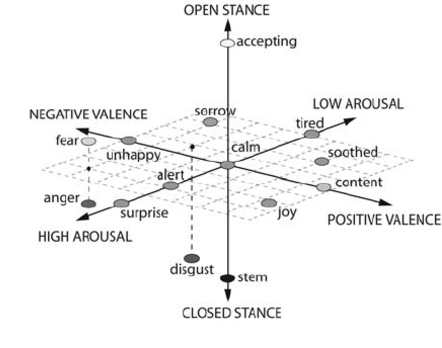
\includegraphics[width=0.9\columnwidth]{res/fig/pad-model-3D}
\caption{Modelul PAD 3D de clasificare a emoțiilor \cite{b7}}
\label{fig1}
\end{figure}

Din acest model se disting următoarele:

\begin{itemize}
\item Excitarea(Arousal) - emoțiile sunt caracterizate pe baza nivelului lor de excitare. 

\item Valență - emoțiile sunt caracterizate în funcție de cât sunt de pozitive sau de negative. Emoțiile pozitive sporesc atenția și alte funcții cognitive ale unei persoane
\end{itemize}


\section{Caracteristici utilizate pentru recunoașterea emoțiilor}
Pentru realizarea unui sistem de recunoaștere a emoțiilor din vorbirea unui subiect este necesară identificarea caracteristicilor ce caracterizează diversele emoții. O alegerea caracteristicilor va influența performanțele sistemului.

Pentru o analiză eficientă a caracteristicilor trebuie să se țină seama de regiunea de analiză utilizată pentru extragerea caracteristicilor, să se aleagă caracteristica potrivită pentru identificarea emoției, să se ia în calcul efectele proceselor uzuale de procesare a semnalului vocal cum ar fi filtrarea și eliminarea zonelor de liniște dar și de asemenea să se ia în calcul faptul că trăsăturile acustice s-ar putea să nu fie suficiente pentru modelarea emoțiilor și că ar putea să se folosească și alte tipuri de caracteristici cum ar fi informația discursului sau trăsăturile faciale. În continuare vor fi detaliate aceste aspecte.


\subsection{Caracteristici locale și caracteristici globale}
Primul aspect se referă la selectarea regiunii de analiză folosită pentru extragerea caracteristicilor. Aici există două abordări. Divizarea semnalului în cadre de durată scurtă pentru care se calculează vectorul caracteristic sau extragerea de mărimi statistice globale pentru întreaga propoziție. 

Deoarece semnalul vocal este nestaționar, se practică divizarea acestuia în ferestre mici de 20 până la 40 de ms. O caracteristică importantă a semnalului vocal, care facilitează analiza acestuia este că acesta este aproximativ staționar pe perioade scurte de timp. Din fiecare astfel de fereastră sunt extrase caracteristici prozodice cum ar fi frecvența fundamentală și energia și denumite caracteristici locale. 

Pe de altă parte, caracteristicile globale reprezintă statistici ale tuturor caracteristicilor locale extrase din mesaj. Majoritatea cercetătorilor au agreat faptul că aceste caracteristici globale sunt superioare caracteristicilor locale din punct de vedere al preciziei și a timpului de clasificare. Caracteristicile globale mai au încă un avantaj față de cele locale și anume acela că sunt mult mai puține la număr, ceea ce facilitează o execuție mult mai rapidă a unor algoritmi cum ar fi cel de ”validare în cruce”. Algoritmul de validare în cruce reprezintă o tehnică de evaluare a modelelor predictive petiționând mostra originală într-un set de antrenare pentru antrenarea modelului și un set de evaluare \cite{b2}. Utilizarea acestora este eficientă doar în cazul distingerii emoțiilor de excitație înaltă (ex. furia, frica și bucuria) de cele de excitare joasă(ex. tristețea). Caracteristicile globale nu reușesc să realizeze o clasificare precisă a emoțiilor cu excitare similară de exemplu identificarea furiei față de bucurie. De asemenea, mai prezintă și dezavantajul că informația temporală prezentă în mesaj este pierdută. Și încă un dezavantaj îl reprezintă chiar faptul că sunt într-un număr mai mic decât caracteristicile locale deoarece s-ar putea să nu se poată antrena modele de tipul HMM sau SVM.

O altă abordare pentru extragerea de caracteristici o reprezintă segmentarea semnalului pe durate scurte pentru analiza fonemelor. Această abordare se bazează pe faptul că forma spectrului fonemelor variază în funcție de emoții. Această afirmație este valabilă doar pentru vocale.


\subsection{Clasificarea caracteristicilor}
Un aspect important în recunoașterea emoțiilor îl reprezintă extragerea caracteristicilor semnalului vocal care caracterizează eficient emoția din mesaj dar în același timp este independentă de vorbitor sau de conținutul lexical.

Caracteristicile vorbirii pot fi grupate în următoarele categorii: Caracteristici continue, caracteristici calitative, caracteristici spectrale și caracteristici bazate pe operatorul TEO. În figura 1 se pot observa exemple de caracteristici aparținând fiecărei categorii.

\begin{figure}[htb]
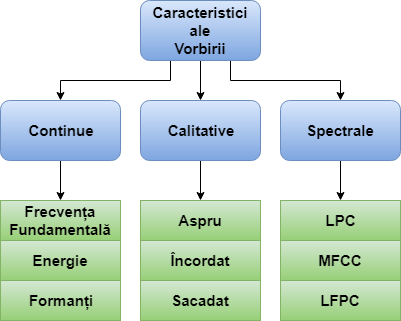
\includegraphics[width=0.85\columnwidth]{res/fig/clasificare-caracteristicilor}
\caption{Categorii de caracteristici ale semnalelor vocale}
\label{fig2}
\end{figure}

\subsubsection{Caracteristici de vorbire continue}
Caracteristicile prozodice continue cum ar fi frecvența fundamentală și energia exprimă o mare parte din sentimentele existente într-un mesaj. S-a observat că starea de excitare a subiectului influențează distribuția spectrală a energiei precum și frecvența și durata pauzelor din vorbire. Conform studiilor, aceste caracteristici acustice pot fi grupate în \cite{b1}:

\begin{itemize}
\item Caracteristici asociate frecvenței fundamentale;

\item Caracteristici bazate pe formanți

\item Caracteristici asociate energiei semnalului vocal

\item Caracteristici ale articulării
\end{itemize}


\subsubsection{Caracteristici de calitate a vocii}
Calitatea vocii este strâns legată de tipurile de emoții, aceasta este descrisă de emoții care direcționează puternic subiecții către un șir de acțiuni. Acestea sunt opuse emoțiilor fundamentale care influențează pozitiv sau negativ acțiunile și gândurile unei persoane. O gamă largă de variabile fonetice contribuie la impresia subiectivă de calitate a vocii. Corelațiile acustice sunt grupate în următoarele categorii \cite{b1}:

\begin{itemize}
\item Nivelul vocii, amplitudinea semnalului, energia și durata s-au dovedit a fi metrici bune pentru nivelul vocii.

\item Frecvența fundamentală a vocii

\item Fraze, foneme, cuvinte

\item Structurile temporale
\end{itemize}


\subsubsection{Caracteristici bazate pe spectru}
Acestea sunt adesea reprezentări ale semnalului pe perioade scurte de timp. Emoțiile dintr-un mesaj influențează distribuția spectrală de energie a mesajului. De exemplu, mesajele care sunt rostite când subiectul este fericit au un nivel ridicat al energiei pentru frecvențele înalte pe când cele rostite de subiecți care sunt triști emoțional au nivele scăzute ale energiei pentru aceleași frecvențe. 
Pentru o mai bună exploatare a gamei de frecvențe, spectrul este trecut printr-o serie de filtre trece-bandă. Caracteristicile spectrale sunt extrase pe baza rezultatelor obținute de la fiecare filtru. Deoarece percepția umană a frecvenței fundamentale nu este modelată liniar, filtrele trece-bandă sunt distribuite uniform cu privire la o  metodă neliniară potrivită cum ar fi scala frecvențelor Mel. 


\subsection{Procesarea vorbirii}
Înaintea extragerii caracteristicilor este necesară o preprocesare a semnalului audio. De exemplu, datorită diferențelor din mediul de înregistrare este necesară o normalizare a energiei pentru toate mesajele. Alt exemplu îl reprezintă netezirea contururilor extrase, pentru aceasta se folosește metoda suprapunerii cadrelor. Pentru eliminarea ondulațiilor din spectrul de frecvențe sunt utilizate ferestre de tip Hamming.

Deoarece intervalele de liniște pot oferi informații importante asupra stării emoționale, acestea sunt păstrate intacte, față de procesele normale de analiză a vorbirii.

Odată extrase caracteristicile se poate să fie necesară o postprocesare înainte de a antrena clasificatorul. De exemplu, este posibil ca vectorii extrași să aibă unități diferite și prin urmare, valorile lor numerice pot avea ordine de mărime diferite sau pot lipsi cu desăvârșire.


\subsection{Combinarea caracteristicilor acustice cu alte surse de informații}
În multe situații, nu este suficientă doar informația provenită din semnalul vocal. Se pot utiliza informațiile referitoare de expresiile faciale sau informația mesajului pentru a putea îmbunătăți performanțele de recunoaștere


\subsubsection{Utilizarea informațiilor acustice și lingvistice}
Semnificația mesajului vorbit este un bun indicator al emoției transmise. Pentru a putea utiliza informațiile lingvistice este necesară recunoașterea secvenței de cuvinte din propoziție. Pentru aceasta este necesar un model de limbă. Acesta descrie constrângerile posibilelor secvențe de cuvinte ale unei limbi. Un astfel de model de limbă este modelul N-gram, acesta atribuie probabilități secvențelor de cuvinte ce pot avea loc. În figura 2 este prezentată arhitectura de bază a unui sistem de recunoaștere a vorbirii ce combină rolurile modelului acustic cu cel al modelului lingvistic pentru identificarea celei mai bune secvențe în care am putea detecta o anumită emoție.

\begin{figure}[htb]
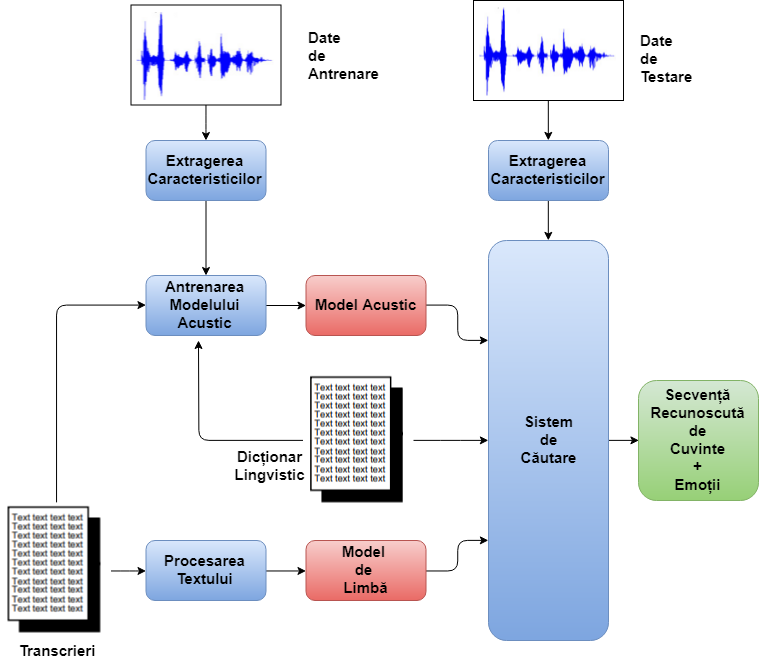
\includegraphics[width=\columnwidth]{res/fig/arhitectura-modelL-modelA}
\caption{Arhitectura unui sistem de recunoaștere a emoțiilor ce utilizează informația acustică și lingvistică}
\label{fig3}
\end{figure}

Modelul de limbă este realizat pe baza transcrierii cuvintelor, în paralel are loc extragerea de vectori de caracteristici din semnalul vocal. Vectorul rezultat împreună cu dicționarul de limbă sunt utilizate pentru a antrena modelele acustice de foneme. La recunoaștere sunt utilizate atât modelul acustic cât și cel de limbă pentru a putea recunoaște secvența după următoarea regulă:

\begin{equation} \label{eq1}
\begin{split}
\hat{W} & =arg \max_{{w}} P(W|Y) = arg \max_{{w}} \frac{P(W)P(Y|W)}{P(Y)} \\
 & =  arg \max_{{w}} P(W)P(Y|W)
\end{split}
\end{equation}

Formula utilizează funcția argmax, care selectează argumentul ce maximizează probabilitatea secvenței de cuvinte. Dezvoltarea din ecuația 1 are la bază regula Bayes și s-a făcut ținând cont de faptul că probabilitatea mesajului vorbit p(X) este independentă de secvența de cuvinte W. Ultimul rezultat evidențiază doi factori care pot fi estimați direct. Problema inițială (găsirea secvenței de cuvinte pe baza mesajului vorbit) a fost împărțită în două sub-probleme mai simple: a) estimarea probabilității apriori a secvenței de cuvinte p(W) și b) estimarea probabilității mesajului vorbit dată fiind secvența de cuvinte pronunțată p(X|W). Primul factor poate fi estimat utilizând exclusiv un model de limbă, iar cel de-al doilea poate fi estimat cu ajutorul unui model acustic. Cele două modele pot fi construite independent așa cum se va vedea în secțiunea următoare, dar vor fi folosite împreună pentru a decoda un mesaj vorbit, așa cum arată ecuația 1 \cite{b3}.

\subsubsection{Utilizarea informațiilor acustice, lingvistice și de discurs}
Indicatorii de discurs reprezintă expresii lingvistice care transmit informații explicite despre structura discursului sau au o contribuție semantică la aceasta. În contextul de recunoaștere a emoțiilor, informațiile legate de discurs mai prezintă și modul în care utilizatorul interacționează cu sistemul. Se întâmplă adesea ca utilizatorul să manifeste emoții in timpul interacțiunii cu sistemul, emoții cum ar fi frustrarea. Informațiile de discurs sunt combinate cu informațiile acustice pentru a îmbunătăți performanțele de recunoaștere.


\section{Metode de recunoaștere a emoțiilor}
În continuare se va prezenta o comparație între rezultatele obținute de două metode de recunoaștere a emoțiilor. Prima metodă se bazează pe utilizarea modele de mixturi Gaussiene antrenate pe baza caracteristicilor globale cum ar fi frecvența fundamentală și conturul energiei semnalului audio. A doua metodă utilizează modele Markov ascunse antrenate pe baza caracteristicilor locale ale semnalului audio. 
De asemenea, vor mai fi prezentați și alți algoritmi utilizați în detecția emoțiilo împreună cu rezultatele obținute.
\subsection{Modele de mixturi Gaussiene}
Modelele de mixturi Gaussiene oferă o bună aproximare a caracteristicilor extrase din semnalul audio prin amestecul ponderat de densități Gaussiene. Coeficienții mixturilor s-au calculat cu ajutorul unui algoritm de maximizare a așteptării. Fiecare emoție este modelata într-un GMM. În experiment s-a remarcat un rezultat bun utilizând un număr de 16 mixturi Gaussiene.

\begin{figure}[htb]
\includegraphics[width=0.8\columnwidth]{res/fig/GMM}
\caption{Matricea de confuzie a analizei utilizând modele GMM \cite{b8}}
\label{fig4}
\end{figure}

 În tabel sunt următoarele abrevieri: sur - surprise, joy - joy, ang - anger, fea - fear, dis - disgust, sad - sadness și ntl - neutral \cite{b8}.



\subsection{Modele Markov ascunse}
Modelul HMM reprezintă un automat cu stări finite alcătuit dintr-un set de stări conectate între care se tranziționează. Secvența de stări a modelului HMM este ascunsă, cu toate
Matricea de confuzie a fost realizată utilizând 64 de stări și patru mixturi Gaussiene. 

\begin{figure}[htb]
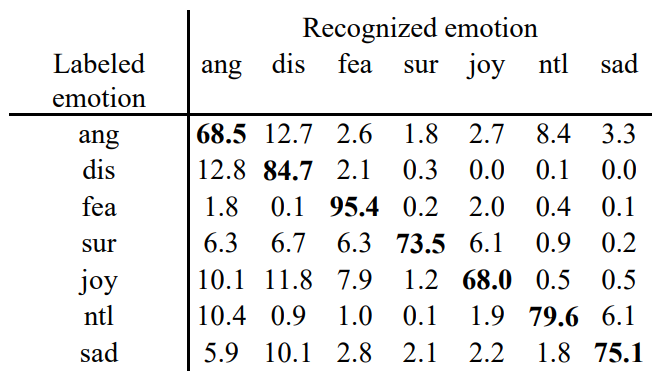
\includegraphics[width=0.8\columnwidth]{res/fig/HMM}
\caption{Matricea de confuzie a analizei utilizând modele HMM \cite{b8}}
\label{fig5}
\end{figure}

În cazul utilizării de modele Markov ascunse s-a obținut o acuratețe medie de $77.8\%$.

În figura 6 este prezentată evoluția ratei de recunoaștere în funcție de numărul de stări folosite. S-a remarcat că cele mai bune rezultate se obțin pentru utilizarea a 64 de stări. 

\begin{figure}[htb]
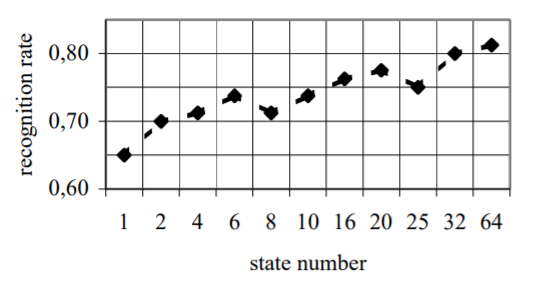
\includegraphics[width=\columnwidth]{res/fig/rata-de-recunoastere-in-functie-de-numarul-de-stari}
\caption{Rata de recunoaștere în funcție de numărul de stări utilizate \cite{b8}}
\label{fig6}
\end{figure}

După cum se poate observa, o creștere generală a performanțelor poate fi obținută crescând numărul de stări. Creșterea performaței vine însă cu un cost și anume creșterea timpului de procesare.


\subsection{K-nearest neighbors}
În procesul de recunoaștere de tipare, k-nearest neighbors reprezintă un algoritm non-parametric folosit pentru clasificare și regresie. Acesta primește ca intrare un număr K de caracteristici de antrenare pe baza cărora poate determina o separare între emoții.
În acest caz s-au utilizat 70\% din setul de date s70 pentru antrenare și 30\% dintre ele ca set de test. Pentur K varian între 1 și 15 s-au obținut următoarele rezultate de precizie: Pentru utilizarea a 8 caracteristici s-a obținut o acuratețe medie aproximativ egală cu 55\%, în cazul utilizării a 10 și 14 caracteristici se obține un rezultat mult mai mare al detecției de furie și anume 65\%. Se obțin rezultate slabe în cazul recunoașterii fricii (13\%, 7\% și 1\% pentru un număr de 8, 10 respectiv 14 caracteristici).

\begin{figure}[htb]
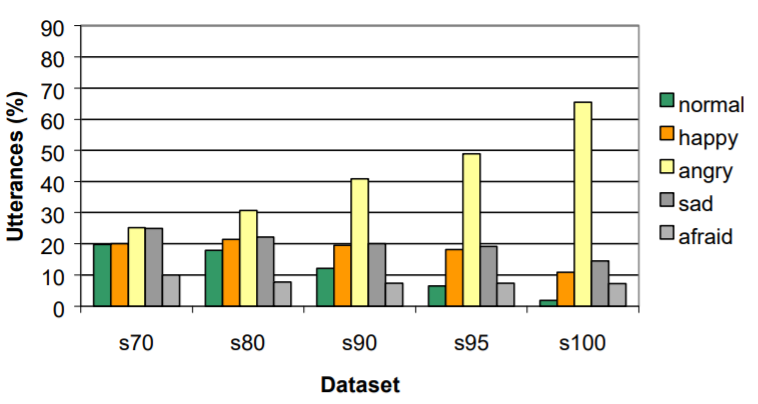
\includegraphics[width=\columnwidth]{res/fig/data-set}
\caption{Distribuția emoțiilor pentur setul de date \cite{b9}}
\label{fig7}
\end{figure}


\subsection{Rețele neuronale}
S-a utilizat o reșea cu două niveluri cu un vector de intrare de 8, 10 respectiv 14 elemente, 10 sau 20 de noduri în nivelul ascuns și 5 noduri ăn nivelul liniar de ieșire. Numărul de intrari corespunde numărului de caracteristici iar numărul de ieșiri corespunde numărului de emoții. Pentur antrenarea acestei rețele s-au utilizat seturile de date s70, s80 și s90 care au fost împărțite în 70\% date de antrenare și 30\% date de testare. Au fost create mai multe clasificatoare ce au fost antrenate cu matrici de ponderare diferite. Această abordare a fost aplicată pe setul de date s70 pentru 8 caracteristici. S-au obșinut următoarele rezultate: 

\begin{table}[htb]
\centering
\caption{Rezultate obținute în cazul recunoașterii de emoții cu ajutorul rețelelor neuronale}
\label{table1}
\setlength{\tabcolsep}{3pt}
\begin{tabular}{|p{0.25\columnwidth}|p{0.25\columnwidth}|}
\hline


Acuratețe&
Emoție\\
\hline

Stare normală&
55-65\%\\
\hline

Fericire&
60-70\%\\
\hline

Furie&
60-80\%\\
\hline

Frică&
25-50\%\\
\hline

Acuratețe medie&
65\%\\
\hline

\end{tabular}
\label{tab1}
\end{table}


\subsection{Ansamblu de rețele neuronale}
Un ansamblu de rețele neuronale este compus dintr-un număr impar de clasificatoare ce au fost antrenate pe diferite subseturi de date folosind agregare bootstrap dar și tehnici de validare în cruce. Deciziile se iau pe baza principiului de vot majoritar. Numărul de rețele reuronale din ansamblu a fost variat într 7 și 15. În figura 8 este prezentată acuratețea de recunoaștere medie a ansamblului format din 15 rețele neuronale. S-a utulizat setul de date s70, numărul de caracteristici utilizate este de 8, 10 respectiv 14 și s-a ținut cont și de cele două arhitecturi cu 10 respectiv 20 de neuroni în nivelul ascuns.

\begin{figure}[htb]
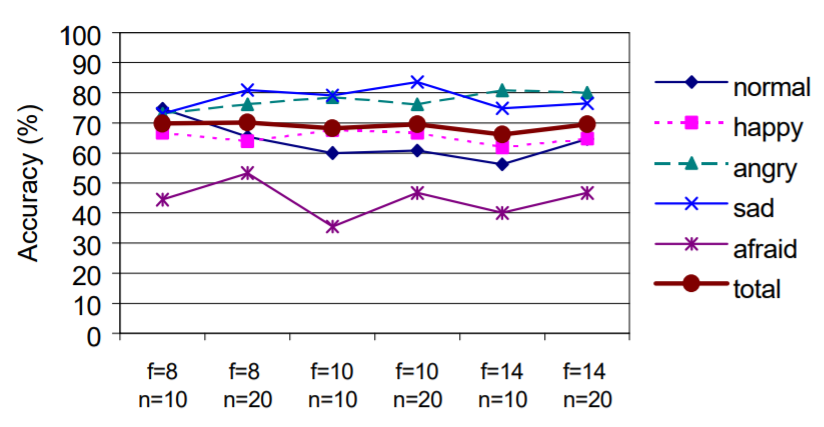
\includegraphics[width=\columnwidth]{res/fig/precizia-medie-a-recunoasterii-emotiilor}
\caption{Acuratețea recunoașterii emoțiilor pentru setul de date s70 \cite{b9}}
\label{fig8}
\end{figure}

Se poate observa din grafic că acuratețea cu care se efectuează detecția fericirii își păstrează valoarea pe la aproximativ 65\% pentru toate cazurile de variere a caracteristicilor de intrare sau a arhitecturilor. Acuratețea pentru detecția fricii este relativ scăzută, aceasta este identificată cu o precizie de 35-53\%. Precizia detecției furiei pornește de la 73\% pentru un vector de 8 caracteristici și crește până la 81\% pentur un set de 14 caracteristici. Cel mai bun rezultat din punct de vedere al acurateții îl reprezintă detecția tristeții, aceasta având o precizie de 73\% to 83\%. Acuratețea medie este situată la 70\%. 


\section{Concluzii}
În acest document au fost prezentate câteva aplicații practice în care poate fi utilizat procesul de recunoaștere a emoțiilor pe baza semnalului vocal. De asemena au mai fost prezentate și principalele caracteristici pe baza cărora se face analiza semnalului și s-au prezentat rezultatele obținute în cazul utilizării a două metode distincte de recunoaștere a emoțiilor.Ambele metode prezentate s-au dovedit a fi capabile să identifice emoțiile din mesaje audio vocale. Tabelele de confuzie arată clar că unele emoții sunt confundate între ele, ceea ce indică similitudini între caracteristicile emoțiilor. De asemenea, aceste rezultate din tabelul de confuzie mai pot fi influențate și de faptul că datele utilizate la antrenare nu au avut cea mai bună calitate din punctul de vedere al calității emoțiilor. Din cele două tabele se remarcă faptul că utilizarea caracteristicilor globale oferă rezultate mai bune decât utilizarea caracteristicilor locale. 

\begin{thebibliography}{00}

\bibitem{b1} https://www.internetworldstats.com/stats.htm

\bibitem{b2} L. F. Coppenrath and Associates. „Biopassword Technology Overview”, http://www.lfca.net/Reference\%20Documents/Biometric\%20Solutions\%20By\%20Classification.pdf

\bibitem{b3} Horia Cucu: ``Proiect de cercetare-dezvoltare în Tehnologia Vorbirii''

\bibitem{b4} Senaka Amarakeerthi, Rasika Ranaweera, and Michael Cohen: ``Speech-based Emotion Characterization using Postures and Gestures in CVEs'', Cyberworlds (CW), 2010 International Conference, 20-22 Oct. 2010.

\bibitem{b5} Vicki R. LeBlanc, Meghan M. McConnell, Sandra D. Monteiro: ``Predictable chaos: a review of the effects of emotions on attention, memory and decision making'', Adv Health Sci Educ Theory Pract. 2015 Mar; 20(1):265-82.

\bibitem{b6} Paul Ekman: ``Emotions Revealed''

\bibitem{b7} Jonghwa Kim, Elisabeth Andre: ``Emotion Recognition Based on Physiological Changes in Music Listening'',  IEEE Transactions on Pattern Analysis and Machine Intelligence ( Volume: 30, Issue: 12, Dec. 2008 ), 02 February 2008, 2067 - 2083

\bibitem{b8} Björn Schuller, Gerhard Rigoll, and Manfred Lang: ``HIDDEN MARKOV MODEL-BASED SPEECH EMOTION RECOGNITION'', Multimedia and Expo, 2003. ICME '03. Proceedings. 2003 International Conference,  6-9 July 2003.

\bibitem{b9} Valery A. Petrushin: ``EMOTION RECOGNITION IN SPEECH SIGNAL:
EXPERIMENTAL STUDY, DEVELOPMENT, AND APPLICATION'', International Conference on Spoken Language Processing (ICSLP 2000)

\end{thebibliography}
\end{document}
